\label{chap:implementation}
%FIXME: V1 decoder logic
%FIXME: original SCB
%FIXME: Add information about the development history thingies from the repo
%FIXME: my research group's arrays?
%FIXME: talk about fw control modularity

%FIXME: fix this paragraph
This chapter describes an FPGA implementation of the PDP architecture~\cite{LandwehrEtAl2019_2,JacksonEtAl2019,BrowningEtAl2020}. For the purposes of this discussion, only relevant details are included to ease the readers understanding. First, the chapter will discuss the purpose of the implemented architecture. Following this each component will be discussed at a high-level. Finally, the operation of sub-components will be discussed.

\section{HDMI Transport Layer}
    \label{sec:hdmi_transport_layer}
    %FIXME: Discuss goal 4

    This section discusses utilizing HDMI as a transport layer for the PDP. HDMI was chosen for the first implementation of the PDP for several reasons. Firstly, current IRSP technology typically utilizes display protocols and the cooresponding links so from the perspective of hardware compatibility a display based protocol layer is ideal. Secondly, providing a backwards compatible implementation of the PDP is a design goal as discussed in Chapter~\ref{sec:design_methodology}. Thirdly, utilizing existing hardware and systems is much cheaper and quicker than designing new hardware. Fourthly, minimizing barriers to entry for users of the protocol is important. Fifthly, it allows for a direct comparison with the same hardware. Sixthly, the systems in my lab utilize HDMI directly already.

    Recall that HDMI is a display protocol with blanking regions as discussed extensively in Chapter~\ref{sec:conventional_display_protocols}. Display protocols have an {\it Active Video} region as shown in Figure~\ref{fig:display_protocol_timing_overview}. This region is made up of scanlines that represent rows of pixels. In normal HDMI operation, the active video region is is simply representation of all visible pixels for a projector to display similar to when HDMI is utilized with a normal computer monitor. At the start of a frame, the first pixel will be streamed to an HDMI decoder and translated to an analog voltage to physically drive the first pixel of a display starting from the top left corner. Following this, subsequent pixels as streamed in and drive each pixel moving toward the right. When an hsync pulse occurs, the display moves to the next row and begins again. this is a typical rasterisation process.

    Traditional IRSP technology uses display protocols quite similarly but reorders data depending on how the rasterization process differs for the projector hardware. Recall the NSLEDS and HDILED array write process discussed in Chapter~\ref{sec:array_Interleaved_write_process} which includes a transpose and data reordering. For purposes of this discussion let us put aside any data reordering and blanking regions. Without lost of generality, drawing to an IRSP looks like Figure~\ref{fig:classic_video} where {\it D} represents an individual 24-bit pixel. Each {\it D} pixel would be decoded one by one as the data is streamed over HDMI to a decoder, and mapped to physical pixel on an array.

    \begin{figure}
        \centering
        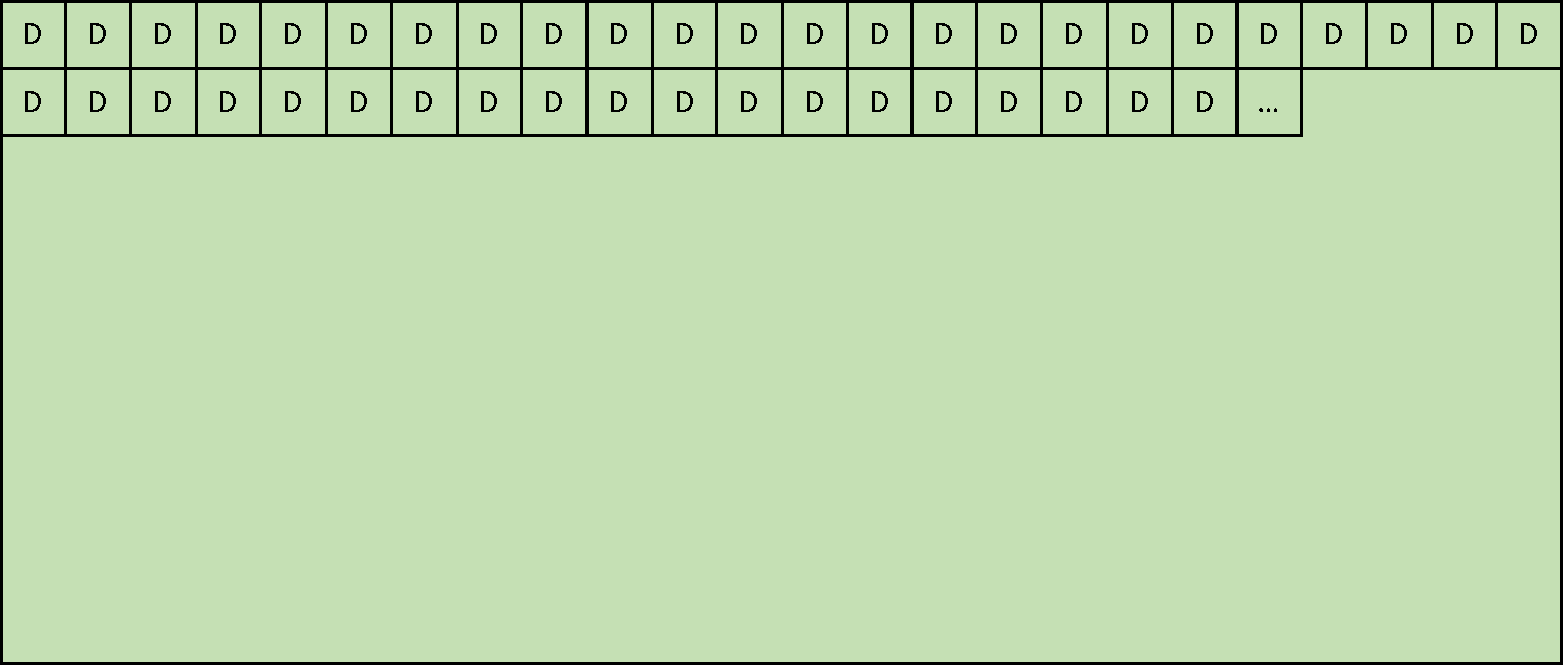
\includegraphics[width=1.0\textwidth]{fig/classic_video.pdf}
        \caption{Normal Frame with Display Data}
        \label{fig:classic_video}
    \end{figure}

    Now let us review the details of the PDP {\it Draw Region} packet shown in Figure~\ref{fig:packet_refresher}. Recall that it consist of an ID number, x start address, x end address, y start address, end y address, and trailing pixel data. The header data is denoted in yellow and the pixel data denoted in green. Recall additionally, that the PDP allows its internal word size to be implementation specific; as such, for HDMI it is ideal to use a 24-bit word size in order to allow for fixed width pixel decoder logic. Additionally, this allows for each PDP word to be directly embeddable within an HDMI display stream with a one to one mapping between an HDMI pixel and a PDP word.

    \begin{figure}
        \centering
        
\includegraphics[width=0.5\textwidth]{fig/packet_refresher.pdf}
        \caption{Draw Region Packet}
        \label{fig:packet_refresher}
    \end{figure}

    Extrapolating, PDP region packets can be embedded into a HDMI data stream as shown in Figure~\ref{fig:embedded_frame} where each PDP word would be represented as a 24-bit pixel in the HDMI data stream. However, the meaning of the pixels differs from a normal frame in that only some pixels will be displayed to an array, and the location of displayed pixels is dependent on the header data preceding the pixels instead of using the start of the frame and the hsync regions to determine the location as is the case with normal HDMI. As the pixel words are streamed in, they are decoded one by one and examined for a context. For example, at the start of the example stream, an ID word would be streamed and decoded, signaling to the firmware that a Draw Region packet is being streamed in. From there, the four header words representing the region size would be streamed in, and stored for determining where to draw the pixel data that follows. As the pixel data is streamed in, the firmware would actively draw pixels in the cooresponding locations on the array where the header says the data should be located. This process would be continued until the end of a packet, and then the subsequent packet would undergo the same process.

    \begin{figure}
        \centering
        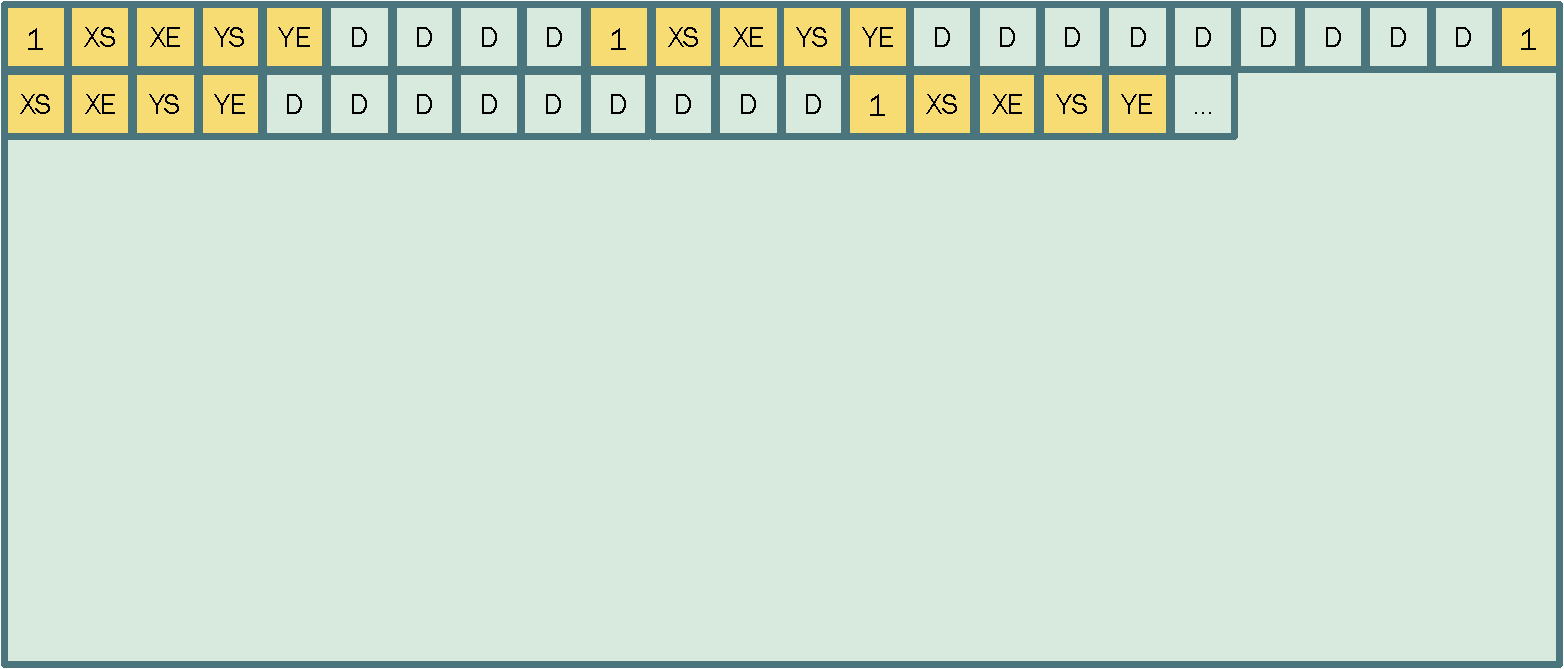
\includegraphics[width=1.0\textwidth]{fig/embedded_frame.pdf}
        \caption{Embedded PDP Frame}
        \label{fig:embedded_frame}
    \end{figure}

    This effectively separates the location a pixel is drawn at from the location in which it exist within an HDMI stream allowing for pixels to be driven independently of the HDMI stream resolution. Moreover, pixels can be driven more than one time within an embedded PDP frame by simply specifying another packet with the same overlapping locations. This allows for pixels to be driven at a faster rate then the base HDMI resolution. In fact, with the separation of pixel draw location from stream location, a specific HDMI resolution is not even necessary. Smaller faster resolutions can be utilized to draw arrays with larger resolutions than a modeline specifies as shown in Figure~\ref{fig:embedded_frame_to_emitter}. Ultimately, this allows for costume tailored modelines with different resolutions and base frame rates to be utilizable with the PDP over HDMI. Moreover, these benefits would hold for other display protocols if used as a PDP transport layer such as DisplayPort, and would allow the PDP to be utilized by simply replacing the HDMI decoder hardware with other off the shelf decoder components without requiring changes to the PDP decoding logic or implementation, thus easing hardware requirements and vendor lock-in for PDP based implementations.

    \begin{figure}
        \centering
        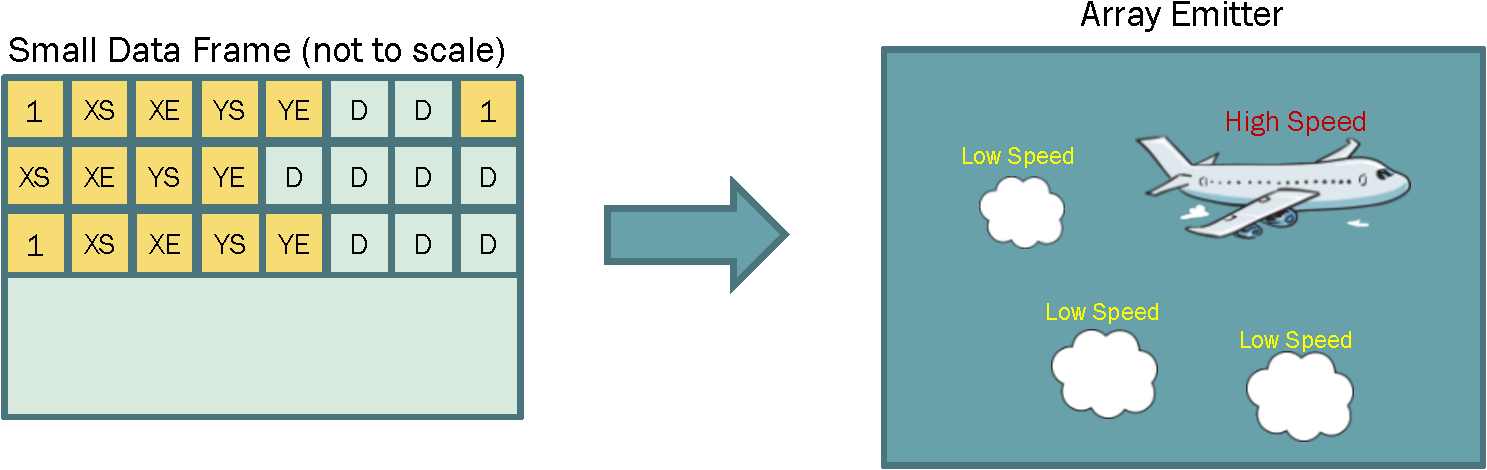
\includegraphics[width=1.0\textwidth]{fig/embedded_frame_to_emitter.pdf}
        \caption{Embedded PDP Frame to Array Mapping}
        \label{fig:embedded_frame_to_emitter}
    \end{figure}

    For backwards compatible operation with normal HDMI, one will note that a normal HDMI frame could be expressed as a single draw region packet with a header at the start the start of a frame. For purposes of backwards compatibility it is not necessary to send the header over HDMI itself. Instead, the header information could be sent as configuration information to the PDP firmware and the HDMI data stream treated as normal display data. This allows for the same decoding and array write logic to be used both for embedded PDP frames and normal HDMI frames without requiring a separate implementation. Thus, users can operate the firmware in either a backwards compatible mode of operation or normal PDP mode of operation. Now that the format of data moving into the PDP firmware has been discussed, the next section moves to a general discussion of the PDP firmware layout.

\section{Abstract Architecture}
    There are many important considerations when implementing a PDP based firmware for IRSPs. These range from pulling data into the FPGA over physical pins to clock domain crossing and timing issues.

    HDMI itself operates with a given pixel clock that's specified on the source side of the connection (at the machine generating the HDMI stream), meaning that the PDP firmware needs to support configurable HDMI speeds. The decoding of the HDMI stream itself is performed by off the shelf HDMI cards as noted in Chapter~\ref{sec:close_support_electronics}; therefore, the PDP firmware does not need to directly handle the protocol. Instead the firmware receives individual pixels at the pixel clock rate over two inputs simultaneously due to CSEs having two separate HDMI inputs.

    The array itself requires a specific timing for its signaling as well as enough time to completely settle any analog data lines; otherwise, pixels will flicker due to metastability issues with the signaling. This means that the HDMI clock cannot be directly utilized for timing array writes without introducing severe complications for correct timing. In fact, older non-PDP firmware implementations operated this way which resulted in image quality being negatively impacted at high speeds.

    In order to correct for these issues and guarantee stable operation at high-speed, the PDP firmware implementation instead opted to isolate firmware operation into separate clock domains as shown in Figure~\ref{fig:abstract_architecture}. Ideally, there would simply be write and read clock domains where the write clock domain is clocked by the input HDMI pixel clock, and pixel data is buffered over an asynchronous boundary to the read clock domain. The read clock domain would operate at a static predefined speed that is faster than the write clock domain in order to ensure that under normal operation data cannot be lost. It would be responsible for decoding pixel data into headers and array data and drive an arrays signaling directly. In practice, the writer clock domain is separated into two separate clock domains for each HDMI input so that the HDMI input clocks do not need to be perfectly synchronized. As will be discussed shortly in subsequent sections, a correct and performant asynchronous boundary proved challenging in practice due to metastability issues and varability in FPGA synthesis from build to build.

    \begin{figure}
        \centering
        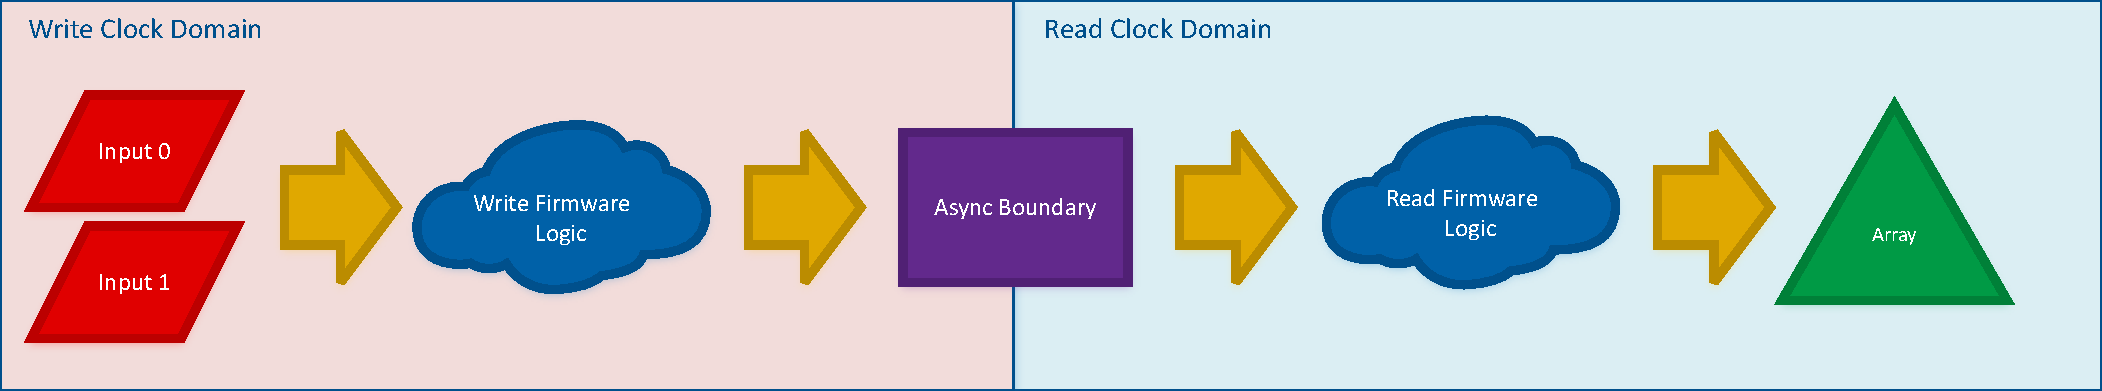
\includegraphics[width=1.0\textwidth]{fig/abstract_architecture.pdf}
        \caption{Abstract PDP Firmware Backend Architecture}
        \label{fig:abstract_architecture}
    \end{figure}

\section{Frontend Architecture}
    \label{sec:frontend_arch}
    This section will discuss the PDP frontend architecture. This is the portion of the firmware that is controllable and allows for user configuration. Recall from Figure~\ref{fig:cse_comm_block} in Chapter~\ref{sec:communication_flow} that CSE communication utilizes the cvorg protocol which is brought into a soft Microblaze soft-processor. The PDP opted to retrofit this layer for its own configuration. Essentially, the frontend architecture works by decoding cvorg protocol commands which in turn set internal PDP registers which are read by the backend architecture for configuration. These include such things as controlling the length of time an individual array write occurs for, controlling delays in the signaling going to an array, and to control whether to operate the firmware in backwards compatibility mode where header data is read from internal PDP registers (called AXI mode) or PDP stream mode where header data is embedded into HDMI streams. Select APIs are shown in Table~\ref{tbl:apis}.

    \begin{table}
        \centering
        \small
        \begin{tabular}{| l l |}
            \hline
            API & Description \\ \hline
            get\_axi\_dimensions     & Gets AXI mode dimensions as 32-bit unsigned integers.        \\
            get\_axi\_mode           & Gets AXI mode. 0 is stream mode. 1 is backwards compat mode. \\
            get\_post\_write\_ticks  & Gets the post write duration for PDP.                        \\
            get\_state               & Gets current firmware state information.                     \\
            get\_write\_ticks        & Gets the delay and duration for pixel writes in PDP.         \\
            set\_axi\_dimensions     & Sets AXI dimensions.                                         \\
            set\_axi\_mode           & Sets AXI mode. 0 is stream mode. 1 is backwards compat mode. \\
            set\_post\_write\_ticks  & Sets the post write duration for PDP.                        \\
            set\_write\_ticks        & Sets the delay and duration for pixel writes in PDP.         \\
            \hline
        \end{tabular}
        \caption{PDP Select Communication APIs}
        \label{tbl:apis}
        %\end{small}
    \end{table}

\section{Overall Backend Architecture}
    \label{sec:backend_arch}
    The implemented backend architecture consists of the portion of the AMM that drives an IRLED tile (or emitter array) directly from data packets sent by a compositor. As such, it is responsible for receiving PDP packets, decoding, validating, and drawing them to an array. This is shown in Figure~\ref{fig:overall_arch}. In the current implementation, packets are sent using an underlying HDMI protocol layer. The incoming data is synchronized across two distinct clock domains utilizing a synchronized circular buffer (SCB). The input side consists of two separate HDMI inputs to meet system bandwidth requirements. Each input is assumed to contain clock skew relative to the other so separate SCBs are used to synchronize these to the system domain. At a high-level, individual data words of 24-bit sized values come in each HDMI clock cycle. These are transitioned to the system domain and stored for retrieval by the array emitter module. The array emitter module is responsible for bringing in each 24-bit word value and emptying the corresponding SCB slot. As it brings in each word, it begins to decode them into PDP commands. Once enough data is buffered for a command, the data is sent to the write buffer module which then drives an emitter directly through I/O lines.

    \begin{figure}
        \centering
        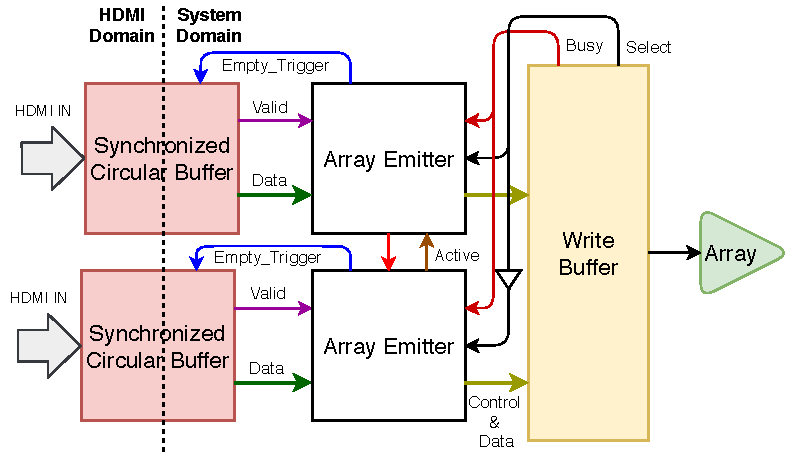
\includegraphics[width=1.0\textwidth]{fig/pdp_overall_arch.pdf}
        \caption{Overall PDP Backend Architecture}
        \label{fig:overall_arch}
    \end{figure}

\section{Synchronized Circular Buffer}

    Figure~\ref{fig:scb_arch} shows the submodule details of the synchronized circular buffer utilized within the implementation. It is used to handle clock domain crossing for data sent from the HDMI domain to the System domain. Internally, it consists of two controllers, two data routers, and the actual internal buffer storage with a built-in synchronizer circuit. The details of each will be explained in following subsections.

    \begin{figure}
        \centering
        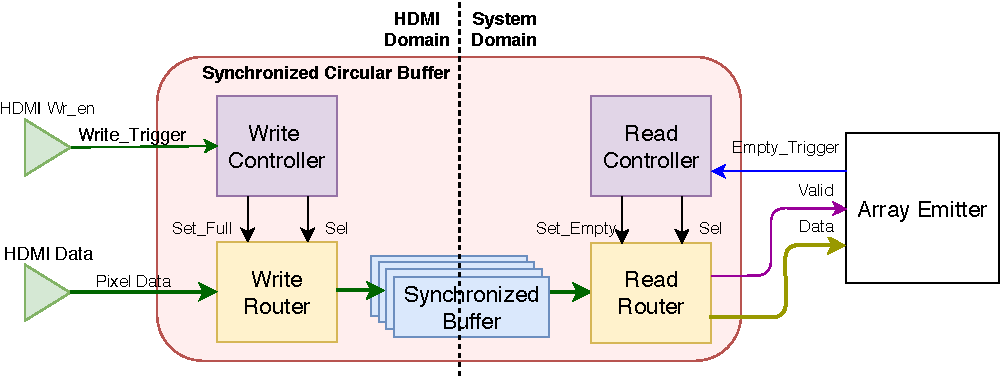
\includegraphics[width=1.0\textwidth]{fig/pdp_scb_arch.pdf}
        \caption{Synchronized Circular Buffer Architecture}
        \label{fig:scb_arch}
    \end{figure}

    \subsection{Controllers}
        The write controller is used to coordinate which internal buffer to write pixel data to. At a given clock cycle, when a pixel is streamed in, the {\it write enable} is used as a {\it write trigger} which causes the write controller to immediately set the current buffer to full, and select the next buffer. On the same clock cycle, the incoming pixel data is stored in the current buffer. In practice, this process repeats for each HDMI clock cycle when write enable is high. The write router performs the actual data redirection based off the buffer selected by the write controller. This will be discussed shortly.

        The read controller behaves similarly to the write controller, but is used to coordinate the reading of stored data from the internal SCB buffers. A {\it valid} signal is used to indicate whether a buffer is filled. If valid is low then the data line output is undefined. In operation, an array emitter will watch for a buffer to be filled then once it is, the array emitter will decode the data and send an {\it empty trigger}, causing the read controller to set the selected buffer to empty and select the next buffer or slot. The array emitter then polls the valid line for the next buffer and the process repeats. The read router performs the actual data redirection based off the {\it select} line controlled by the read controller. This will be discussed shortly.

    \subsection{Routing}
        Figure~\ref{fig:sb_arch} shows the internals of the synchronized buffers used by the SCB with attached data routers. While only four buffers are shown for demonstration purposes, the number of buffers is compile time definable in the implementation. In the system both, both the writer and reader of the buffers have independent views of the the SCB state and data stored within. As mentioned previously, data is mapped based off the select lines. This causes a given buffer's internal lines to be routed in or out depending on the direction of the signals. The {\it empty flag} is used to determine if the buffer is empty. The {\it full flag} is mapped as a {\it valid flag} to the array emitter which uses it to determine if a buffer is full as noted previously. The {\it set\_full} and {\it set\_empty} lines are used simply to change the state of the internal buffers depending on whether they are now empty or full. The {\it hold} lines are used to hold any shift register data when a buffer isn't selected. Any unselected shift register automatically hold their contents. A selected shift register will conditionally hold its contents if a {\it write trigger} is not occuring and update its contents otherwise. Data into the SCB is selectively routed to each shift register to allow for the data to be stored and data out of the SCB is selectively routed to an array emitter for decoding.

        \begin{figure}
            \centering
            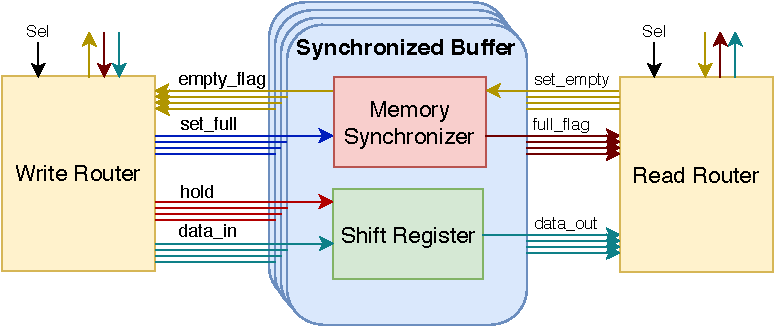
\includegraphics[width=1.0\textwidth]{fig/pdp_sb_arch.pdf}
            \caption{Synchronized Internal Buffer Architecture}
            \label{fig:sb_arch}
        \end{figure}

    \subsection{Internal Buffer and Memory Synchronizer}
        \label{Sec:MemorySync}
        At high-level, internally, a request-acknowledgment handshake is used to ensure the data has transitioned correctly across clock domains and is available on the other side. Once data becomes available, the read router will output the data lines as well as a valid signal indicating that the data can be read and cleared. The read controller will clear it once an empty trigger is sent from the array emitter indicating that the corresponding word has been read. It will then select the next buffer. Once the last buffer is written or read by either controller, the first buffer will be selected again.

        Figure~\ref{fig:full_empty_circuit} shows an register-tranfer level (RTL) design of the circuit.

        \begin{figure}
            \centering
            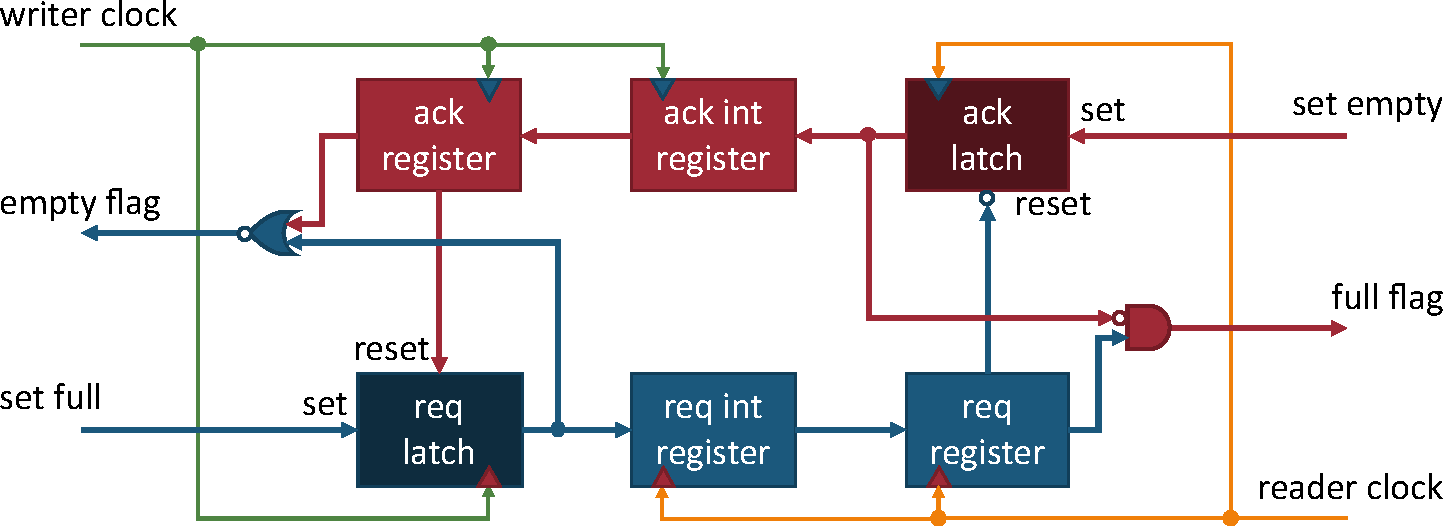
\includegraphics[width=1.0\textwidth]{fig/full_empty_circuit.pdf}
            \caption{Full/Empty Memory Synchronizer Circuit}
            \label{fig:full_empty_circuit}
        \end{figure}
        \begin{minted}[
        frame=lines,
        framesep=2mm,
        baselinestretch=1.0,
        %bgcolor=lightgray,%
        fontsize=\small,
        linenos
        ]{vhdl}
library IEEE;
use IEEE.std_logic_1164.all;
library UNISIM;
use UNISIM.VComponents.all;

entity memory_synchronizer is
    port (
        -- wr domain in:
        wr_reset    : in std_ulogic;         -- global reset
        wr_clk      : in std_ulogic;         -- writer clock
        set_full    : in std_ulogic;         -- writer set_full trigger
        -- wr domain out:
        full_flag   : out std_ulogic := '0'; -- full flag
        -- rd domain in:
        rd_reset    : in std_ulogic;         -- global reset
        rd_clk      : in std_ulogic;         -- reader clock
        set_empty   : in std_ulogic;         -- reader set_empty trigger
        -- rd domain out:
        empty_flag  : out std_ulogic := '1'  -- empty flag
    );
end entity;

architecture Behavioral of memory_synchronizer is
    signal req      : std_ulogic := '0'; -- request writer domain
    signal req_int  : std_ulogic := '0'; -- request buffer
    signal req_reg  : std_ulogic := '0'; -- request reader domain
    signal ack      : std_ulogic := '0'; -- acknowledgement reader domain
    signal ack_int  : std_ulogic := '0'; -- acknowledgement buffer
    signal ack_reg  : std_ulogic := '0'; -- acknowledgement writer domain
begin
    empty_flag <=  req nor ack_reg;
    full_flag <= req_reg and not ack;

    process (wr_clk)
    begin
        if (rising_edge(wr_clk)) then
            -- transition acknowledgement to writer domain.
            ack_int <= ack;
            ack_reg <= ack_int;
            if wr_reset = '1' then
                req <= '0';
                ack_int <= '0';
                ack_reg <= '0';
            else
                if set_full = '1' then  -- set full to signal request.
                    if req = '0' then
                        req <= '1';
                    end if;
                end if;
                if ack_reg = '1' then   -- if reader transitioned ack high
                    req <= '0';         -- then transition request low.
                end if;
            end if;
        end if;
    end process;

    process (rd_clk)
    begin
        if (rising_edge(rd_clk)) then
            -- transition request to reader domain.
            req_int <= req;
            req_reg <= req_int;
            if rd_reset = '1' then
                ack <= '0';
                req_int <= '0';
                req_reg <= '0';
            else
                if set_empty = '1' then -- set empty to signal ack.
                    ack <= '1';
                end if;
                if req_reg = '0' then -- if writer transitioned request low
                    ack <= '0';       -- then transition ack low.
                end if;
            end if;
        end if;
    end process;
end architecture;
        \end{minted}

        %Figure~\ref{blah} shows the internals of the memory synchronizer utilized by the SCB architecture.

\section{Array Emitter}

    Figure~\ref{fig:ae_arch} shows the details of the array emitter module used in the implementation. The logic for handling the PDP is encapsulated completely here. An array emitter module is responsible for decoding the words of the PDP packets and sending pixel data or array reset requests to the write buffer which will either draw to the array or reset the array depending on the requested operation.

    \begin{figure}[t]
        \centering
        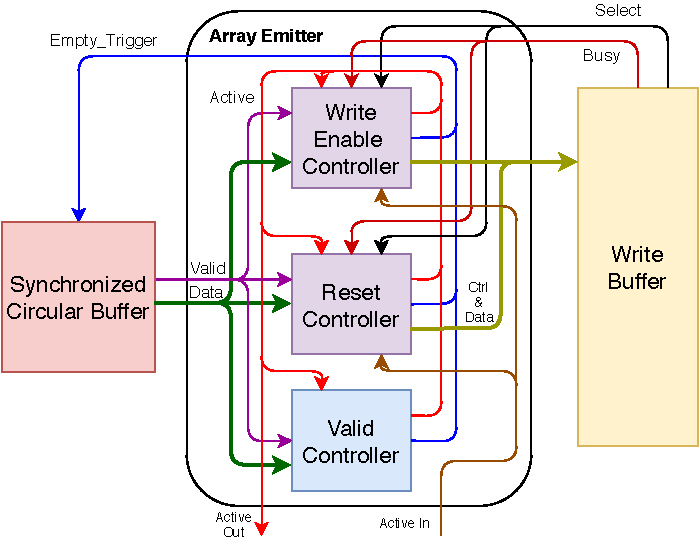
\includegraphics[width=0.95\textwidth]{fig/pdp_ae_arch.pdf}
        \caption{Array Emitter Architecture}
        \label{fig:ae_arch}
    \end{figure}

    Internally, the array emitter consists of individual state machine controllers that each handle a particular packet type. The current implemantion includes a write enable controller, which controls decoding of draw region packets; a reset controller, which controls the array reset process; and a valid controller which does validation checks on the input to verify the correctness of packets discarding any unknown data. For example, unknown packet IDs.

    Each controller takes in similar input signals and produces similar output signals with some exceptions depending on the actual function of the individual controller module. On the input side, each controller takes in a valid and data line corresponding to an individual word of a PDP packet. Additionally, an active line is brought into each controller to indicate whether another controller module is active or not. This is used to ensure that other modules do not become active and attempt to decode data not meant for them while another is currently processing a packet. During an idle phase, the write enable and reset controllers wait for a corresponding packet ID to come in before beginning operation. The details of the state machine will be discussed in the following section.

\section{State Machines}
    \label{sec:state_machines}
    Figure~\ref{fig:state_machine} shows a block diagram of the PDP state machines for the draw region and array reset controllers. Each cycle of the system clock, an array emitter will attempt to read a word of data stored within an SCB. For simplicity, an example draw region packet is shown.

    \begin{figure}[t]
        \centering
        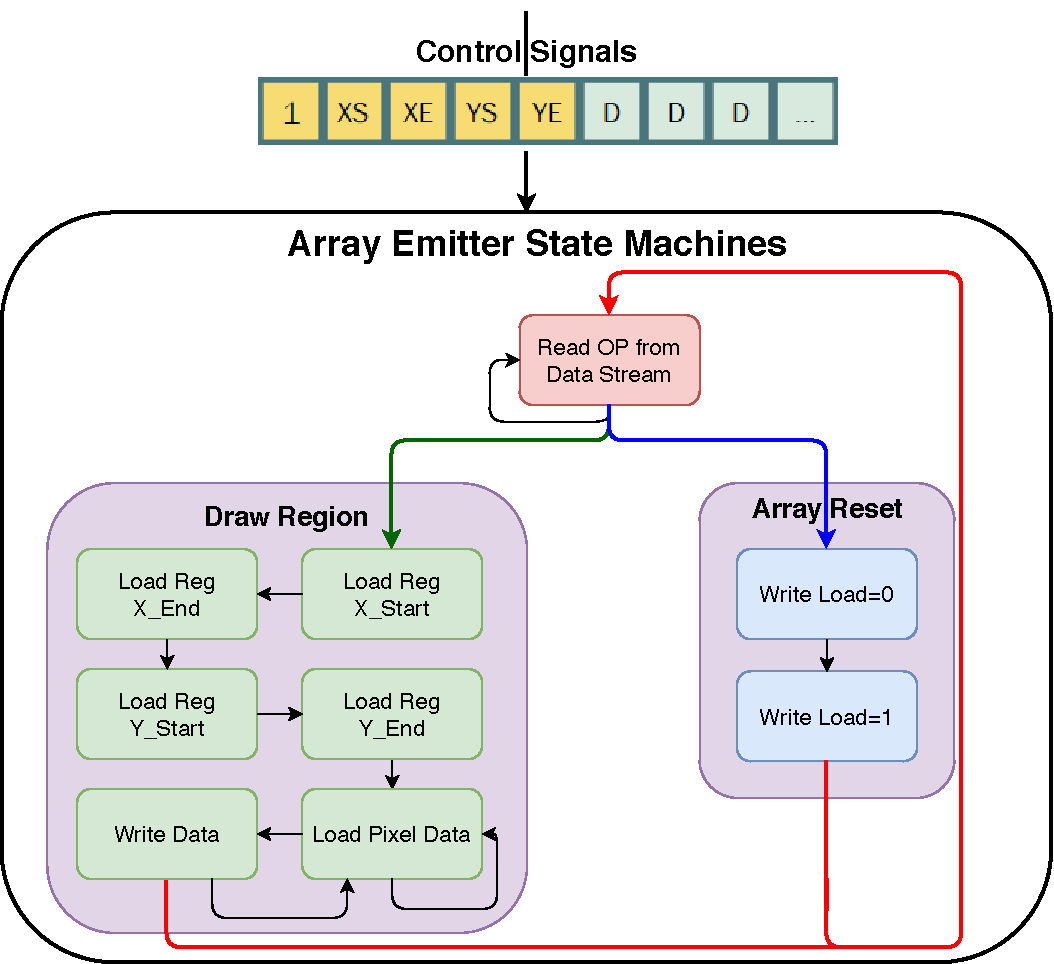
\includegraphics[width=0.95\textwidth]{fig/pdp_state_machine.pdf}
        \caption{PDP State Machine}
        \label{fig:state_machine}
    \end{figure}


    When a packet ID matching an operation handled by a given controller arrives, the corresponding controller will switch states and then wait for the rest of the incoming packet data to arrive. For example, if a draw region packet ID were to arrive, then the state machine would wait for the X start address, X end address, Y start address, and Y end address to arrive word by word by performing a check for valid data each system clock cycle. Finally, after data arrives and the header is decoded, the state machine would load the necessary pixel data for a write and move to the write data state once all data has been buffered. In this state it would send the data to the write buffer. If more data needs to be written for the PDP packet, it would then continue buffering the needed data, and wait for the write buffer to be idle to send the next set of data. This would continue until all data was written for the packet, finally proceeding to the idle state. For more incite, recall that Figure~\ref{fig:pdp_stream} in Chapter~\ref{sec:packet_types} shows an example PDP stream being decoded cycle by cycle. This state machine is simply an implemented version of the decoding process shown there.

    The reset controller contains similar logic. When a packet ID matching a reset packet arrives, the reset controller will begin the array reset process. This is a system specific process but for an NSLEDS array requires enabling all quadrant bits, writing a load signal of 0, and driving the reset signal located on the RIIC high. Following this, it requires enabling all quadrant bits, writing a load signal of 1, and driving the array reset signal to high. The reset controller does this by sending a request for both operations to the write buffer and going back to an idle state afterwards. For more information about these signals see Chapter~\ref{sec:array_Interleaved_write_process}.

    The valid controller (not shown) is used to ensure that incorrect or corrupt packet data is cleared. If an invalid packet command arrives during an array emitter idle phase, the valid controller will simply empty the corresponding SCB slot.

\section{Write Buffer}

    Figure~\ref{fig:wb_arch} shows the details of the write buffer architectures inputs and outputs along with important signaling to other modules. The write buffer is responsible for driving the I/O pins that are passed to the array. At a high level, the write buffer is responsible for coordinating writes between the two array emitters shown. Generally, this is done by handing off write buffer privileges every other write through the Select line in order to ensure starvation does not occur for either HDMI input. The busy line is used to indicate when the write buffer is in the process of writing to the array in order to ensure that array emitter modules do not attempt to send new data to the write buffer while it is currently active.

    \begin{figure}[H]
        \centering
        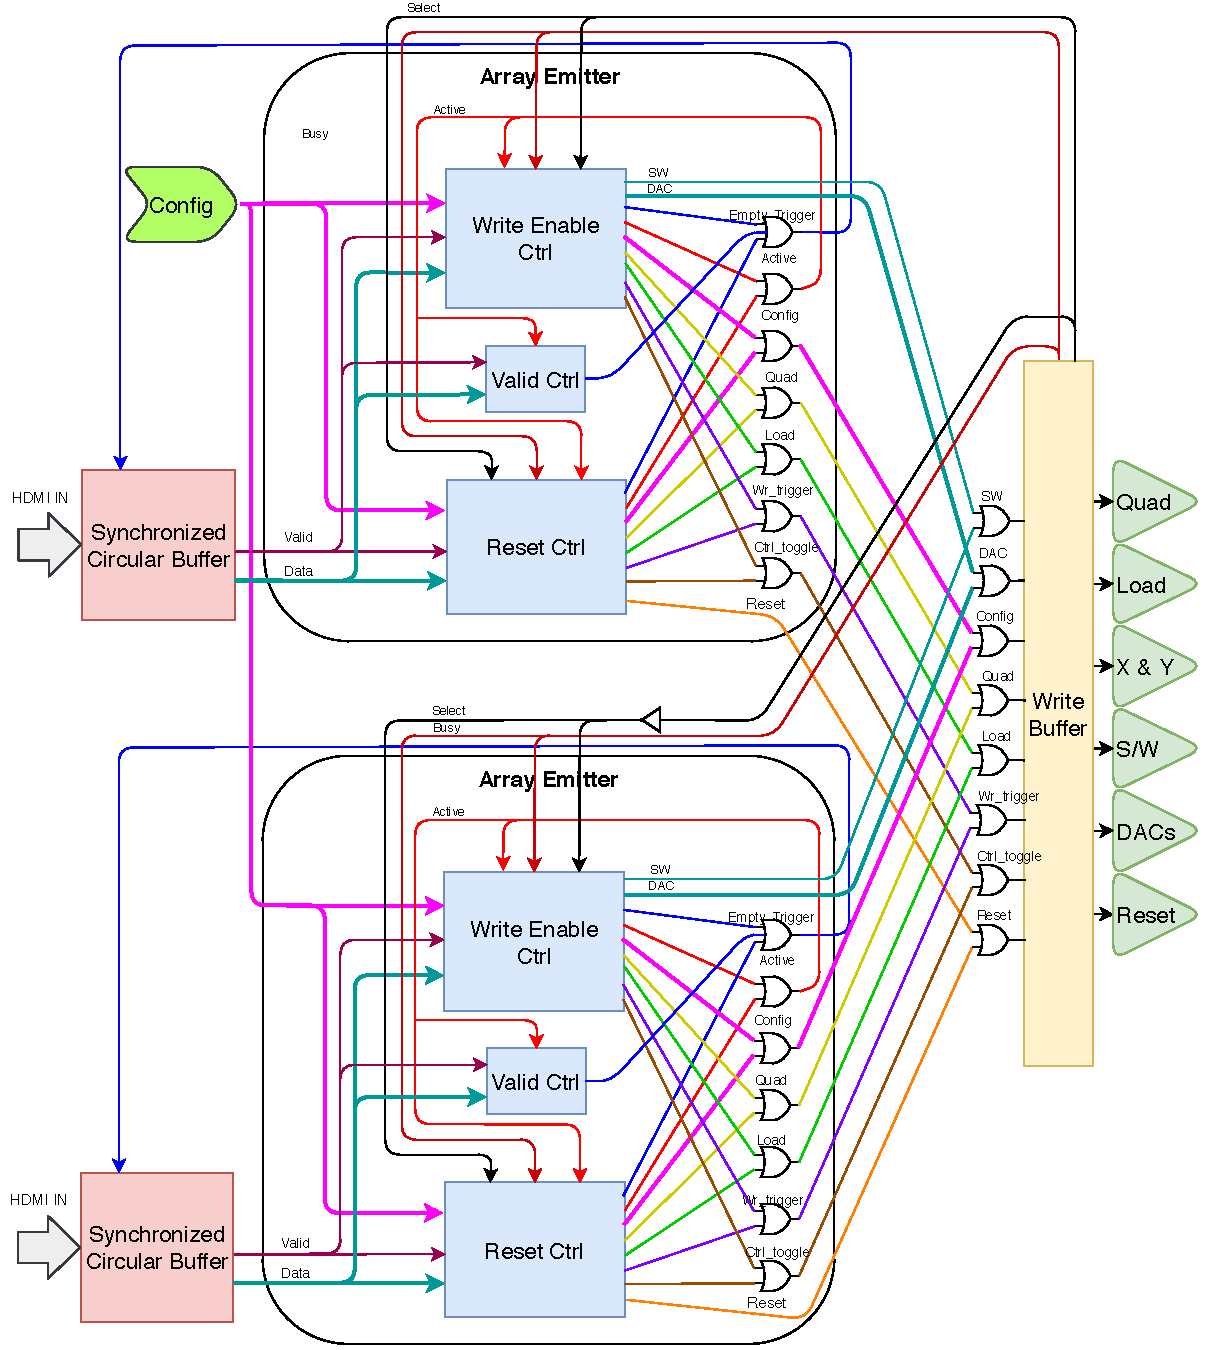
\includegraphics[width=1.0\textwidth]{fig/pdp_wb_arch.pdf}
        \caption{Write Buffer Architecture}
        \label{fig:wb_arch}
    \end{figure}

    For input, the write buffer takes bits representing the signal I/O going to the RIIC. This includes all of the output signals discussed in Chapter~\ref{sec:array_Interleaved_write_process}. Configuration information is sent to indicate for how long a write or reset should occur as well as when during the write process specific signaling should transition high and back to low. These signals are configurable through the frontend APIs discussed in Chapter~\ref{sec:frontend_arch}. It is worth noting that in practice, that this timing is array specific but must be long enough for the analog signaling to settle.
